\section{Введение в вычислительную геометрию}
\begin{center}
    Конспект составил: \textit{Павел Аверин}
\end{center}

\subsection{Геометрические объекты на плоскости}

\subsubsection{Точка}
Точка~--- геометрический объект, не имеющий никаких измеримых характеристик, кроме координат.

Существует несколько систем координат, в которых можно задать точку.

\paragraph{Декартовы координаты}
В декартовой системе координат точка $A$ задаётся парой чисел $(x, y)$ для двумерного пространства, где $x$ и $y$ — это координаты точки по осям $X$ и $Y$ соответственно.

\paragraph{Полярные координаты}
В полярной системе координат точка задаётся парой $(r, \theta)$, где $r$ — это расстояние от начала координат до точки, а $\theta$ — угол, образуемый радиус-вектором с положительной осью $X$. Полярные координаты можно преобразовать в декартовы с помощью следующих формул:

\[
    x = r \cos(\theta), \quad y = r \sin(\theta).
\]

Чтобы преобразовать декартовы координаты обратно в полярные, используются следующие формулы:

\[
    r = \sqrt{x^2 + y^2}, \quad \theta = \arcsin\left(\frac{x}{r}\right).
\]

При вычислении угла $\theta$ необходимо учитывать знак координат $x$ и $y$, чтобы правильно определить четверть, в которой находится точка.

\paragraph*{Пример: Смена системы координат на практике}

Предположим, у нас есть набор точек, расположенных в двумерном пространстве. \newline
\par Мы хотим для данного набора решить задачу кластеризации (задача группировки множества объектов на подмножества (кластеры) таким образом, чтобы объекты из одного кластера были более похожи друг на друга, чем на объекты из других кластеров по какому-либо критерию.)

\begin{figure}[H]
    \centering
    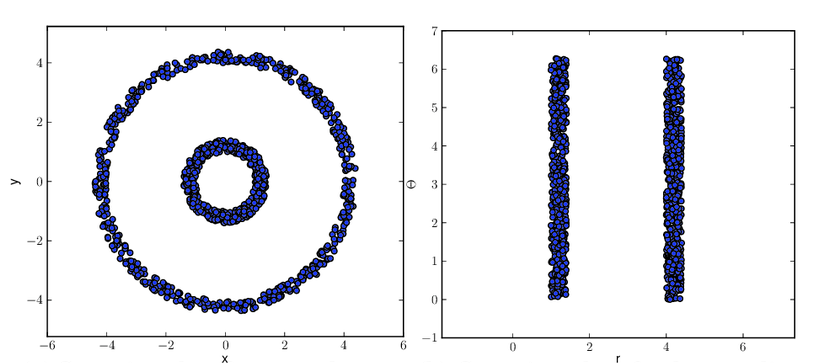
\includegraphics[width = 12cm]{Clusters.png}
    \caption{Слева набор точек в декартовых координатах, справа в полярных}
    \label{fig:float}
\end{figure}

Легко заметить, что при переходе к полярным координатам в данном примере, кластеры явно видны, и задача кластеризации становится тривиальной.

\subsubsection{Прямая}

Прямая — Множество точек, которые лежат на одном уровне и проходят через определённое направление. Имея 2 точки $(x_1, y_1)$, $(x_2, y_2)$, можно задать прямую следующим уравнением:

\[
    ax + by + c = 0
\]

Где коэффициенты $a,b,c$ находятся путём подставления координат точек, которые известны, в уранение.

\paragraph*{Взаимное расположение двух прямых}
Две прямые могут совпадать, пересекаться или быть параллельными.

\( a_1x + b_1y + c_1 = 0 \) и \( a_2x + b_2y + c_2 = 0 \) совпадают, если выполняется следующее условие:

\[
    \frac{a_1}{a_2} = \frac{b_1}{b_2} = \frac{c_1}{c_2}
\]

Если это условие не выполняется, то две прямые либо пересекаются, либо являются параллельными.

Две прямые пересекаются, если они не параллельны, то есть:

\[
    \frac{a_1}{a_2} \neq \frac{b_1}{b_2}
\]

Если же прямые параллельны, то они имеют одинаковые коэффициенты при \(x\) и \(y\), но различные свободные члены. Точка пересечения находится путём решения системы уравнений $(1)$:

\begin{equation}
    \begin{cases}
        a_1 x + b_1 y + c_1 = 0 \\
        a_2 x + b_2 y + c_2 = 0
    \end{cases}\
\end{equation}

\paragraph*{Линейная регрессия} Линейная регрессия -- метод нахождения линейного отношения, который описывает соотношение зависимой и (возможно) независимой переменной.
Говоря другими словами: дан набор точек $(x_1, y_1)...(x_k,y_k)$, требуется провести (регрессионную) прямую $l = f(x)$, минимизирующую функцию
\[
    \left( \sum_{i=1}^{k} \left| y_i - f(x_i) \right|^2 \right)
\]
Т.е прямую с коэффицииентами $a,b,c$, такую что
\[
    \min_{(a, b, c)} \left(\sum_{i=1}^{|k|} \left| y_i - \dfrac{ax_i + c}{b} \right|^2 \right)
\]

\begin{figure}[H]
    \centering
    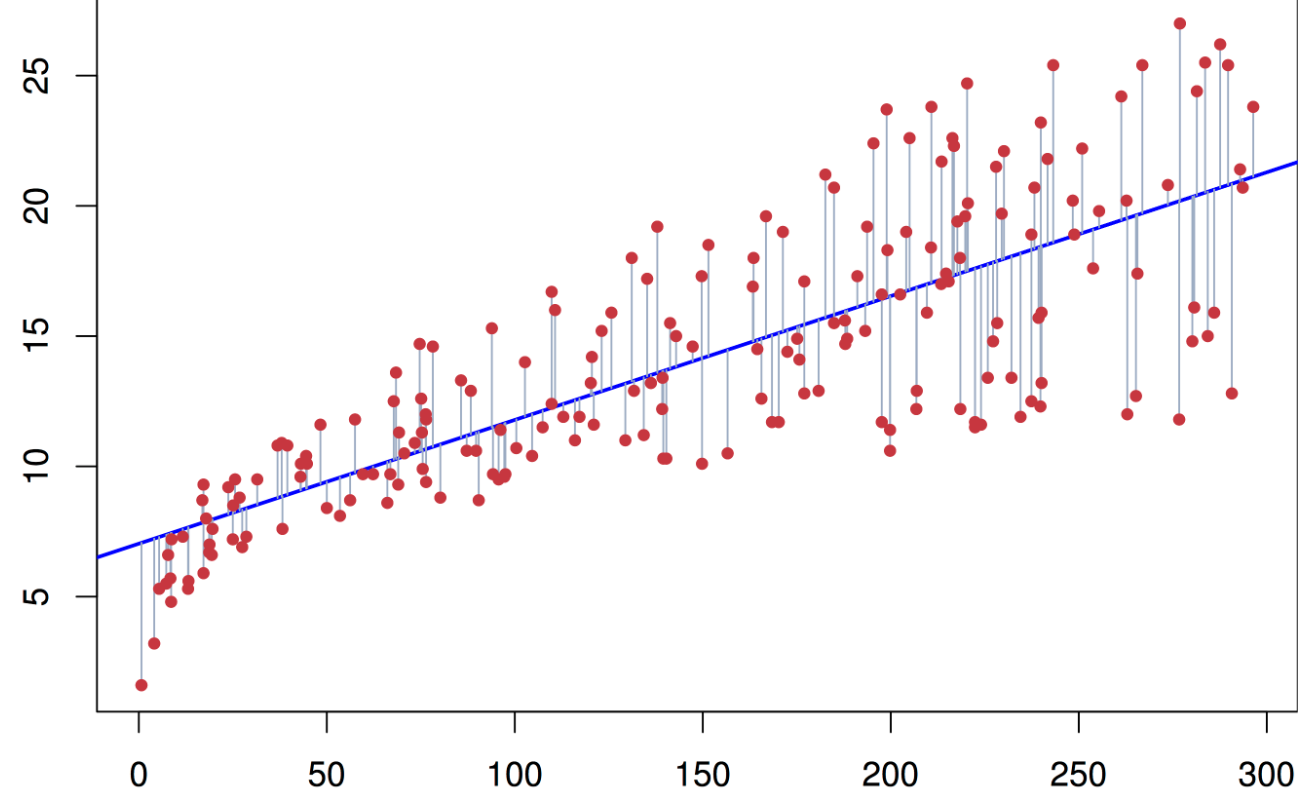
\includegraphics[width = 12cm]{Regression.png}
    \caption{Синяя линяя - проведенная регрессионная прямая}
    \label{fig:float}
\end{figure}

\subsubsection{Окружность}
Окружность - это линия на плоскости, каждая точка которой расположена на одинаковом расстоянии от центра окружности. \newline \newline
Имея центр окружности -- точку $(x_0, y_0)$ и радиус $r$, можно задать окружность с помощью уравнения

\[
    (x - x_0)^2 + (y - y_0)^2 = r^2
\]

\subsubsection{Площадь}

\paragraph*{Площадь треугольника} Пусть даны вектора AB, AC, и их длины, требуется найти площадь (см. Рис 3.)

\begin{figure}[H]
    \centering
    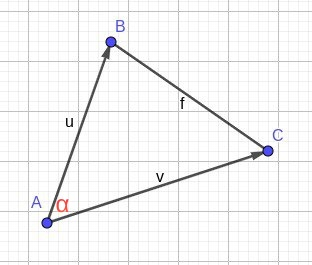
\includegraphics[width = 7cm]{Triangle.jpeg}
    \caption{}
    \label{fig:float}
\end{figure}

Данную задачу можно решать по-разному -- методами школьной геометрии (например, найти длину 3-ей стороны и применить формулу Герона) или с помощью векторного произведения:

\[
    |\vec{ab} \times \vec{ac}| = |\vec{ab}| * |\vec{ac}| * sin(\alpha) = 2 * S_{\Delta ABC}
\]
Что является лучшим вариантом, т.к. векторное произведение можно быстро и эффективно посчитать с помощью матриц.

\paragraph*{Произвольный случай} Если нам дан не треугольник, а произвольная фигура, можно либо пытаться разбить её на треугольники и посчитать их площади (Триангуляция) или взять определенный интеграл (см. Рис. 4)

\begin{figure}[H]
    \centering
    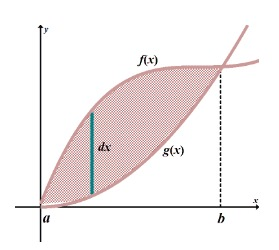
\includegraphics[width = 7cm]{integral.jpeg}
    \caption{Полагаем, что $f(x)$ и $g(x)$ положительные}
    \label{fig:float}
\end{figure}
Площадь фигуры на Рис. 4 можно посчиать по формуле
\[
    \int_a^b (f(x) - g(x)) \, dx
\]

\paragraph*{Численное интегрирование} Под вычисление значений определнных интегралов отведен целый раздел вычислительной математики, рассмотрим метод под названием "Метод прямоугольников"

\begin{figure}[H]
    \centering
    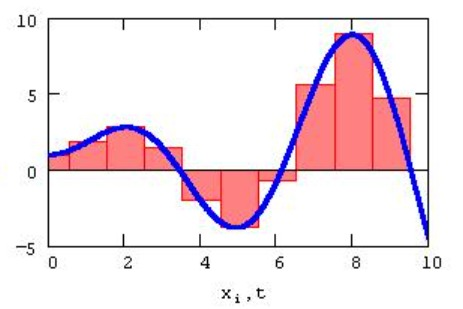
\includegraphics[width = 7cm]{Integral_numerical.jpeg}
    \caption{$a = 0$, $b = 10$}
    \label{fig:float}
\end{figure}
Для подсчета интеграла интервал интегрирования $[a,b]$ разбивается на $N$ отрезков. На каждом из отрезков $f(x)$ заменяется прямоугольником с шириной $h = \dfrac{b - a}{N}$ и высотой $f(x_i)$. При этом точка $x_i$ может выбираться, к примеру, как начало каждого элементарного отрезка, либо как его центр. Формулы прямоугольников для этих двух случаев запишутся в виде

\[
    \left( \sum_{i=0}^{N - 1} \left| f(x_i) \right| \right)
\]

\[
    \left( \sum_{i=0}^{N - 1} \left| f(x_i + \dfrac{h}{2}) \right| \right)
\]

\subsection{Задачи вычислительной геомеотрии}
\subsubsection{Cunvex hull}
Дано множество $n$ точек $X$, Cunvex hull (Выпуклой оболочкой) называется наименьшее выпуклое множество содержащее $X$ (Рис. 5)

\begin{figure}[H]
    \centering
    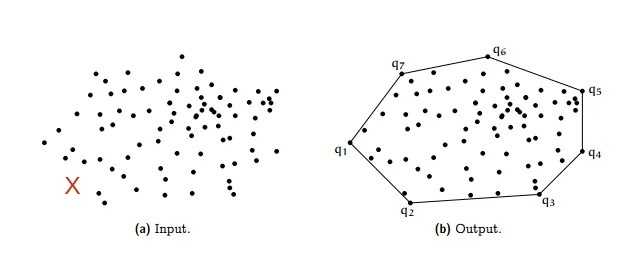
\includegraphics[width = 9cm]{Convex_hull.jpeg}
    \caption{}
    \label{fig:float}
\end{figure}

Прежде чем рассматривать алгоритмы построения выпуклой оболочки, поймем, что данная задача не решается линейно, т.к в противном случае, мы могли бы отсортировать точки по углам

\paragraph*{Алгоритм Джарвиса (Марш Джарвиса)} Очень простой в реализации алгоритм нахождения выпуклой оболочки
\newline \newline
% Алгоритм начинается с $i= 0$ и точки $p_0$, которая попадает на % выпуклую оболочку, т.е ищем за $O(n)$ самую левую точку %сравнивая полярные углы всех точек, относительно точки $p_i$ как %центра координат, затем выбираем точку $p_{i+1}$, такую что, все %другие точки находятся по правую сторону от линии $p_i$$p_{i+1}$. %Далее увеличиваем $i$ на 1 и повторяем процесс до тех пор, пока %$p_0 != p_h$, где $h$ - количество точек на выпуклой оболочке. %Итого сложность данного алгоритма $O(nh)$. Пример работы %изображен на Рис. 6.
1. Возьмем точку $p_0$
нашего множества с самой маленькой $у$-координатой (если таких несколько, берем самую правую из них). Добавляем ее в ответ.  \newline\newline
2. На каждом следующем шаге для последнего добавленного $p_i$
ищем $p_{i+1}$
среди всех недобавленных точек и $p_0$
с максимальным полярным углом относительно $p_i$
(Если углы равны, надо сравнивать по расстоянию). Добавляем $p_{i+1}$
в ответ. Если $p_{i+1}==p_0$
, заканчиваем алгоритм. (На Рис. 7 изображен пример работы алгоритма)
\begin{figure}[H] (На Рис. 7 изображен пример работы алгоритма)
    \centering
    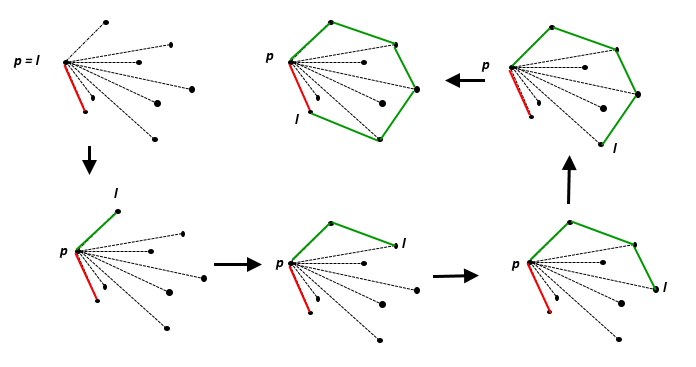
\includegraphics[width = 9cm]{Jarvis.png}
    \caption{}
    \label{fig:float}
\end{figure}

\paragraph*{Алгоритм Грэхэма}
% Алгоритм заключается в том, что мы ищем точки оболочки %последовательно, используя стек.
%\newline \newline
%Находим точку $p_0$ нашего множества с самой маленькой у-%координатой (если таких несколько, берем самую правую из них), %добавляем в ответ. Сортируем все остальные точки по полярному %углу относительно $p_0$.
%Добавляем в ответ самую первую из отсортированных точек $p_1$. 
%Берем следующую по счету точку $t$. Пока $t$ и две последних %точки в текущей оболочке $p_i$ и $p_{i-1}$ образуют неправый %поворот (вектора $p_i$ $t$
% и $p_{i-1}$ $pi$ ), удаляем из оболочки $p_i$.
%Добавляем в оболочку $t$
%. Повторяем процесс пока не закончаться точки
1. Находим точку $p_0$
нашего множества с самой маленькой $у$-координатой (если таких несколько, берем самую правую из них), добавляем в ответ. \newline\newline
2. Сортируем все остальные точки по полярному углу относительно $p_0$
. \newline\newline
3. Добавляем в ответ $p_1$ --- самую первую из отсортированных точек.
4. Берем следующую по счету точку $t$. Пока $t$
и две последних точки в текущей оболочке $p_i$
и $p_{i-1}$
образуют неправый поворот (вектора $p_it$
и $p_{i-1}p_i$
), удаляем из оболочки $p_i$
. \newline\newline
5. Добавляем в оболочку $t$
.\newline\newline
6. Делаем п.4, пока не закончатся точки.
\begin{figure}[H]
    \centering
    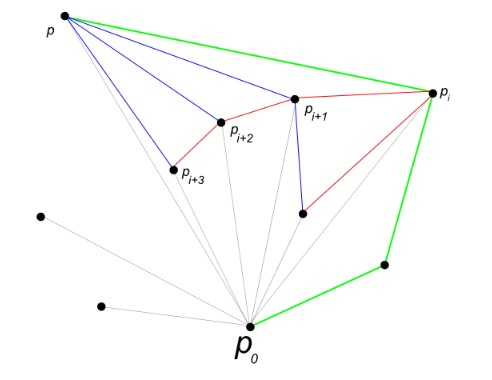
\includegraphics[width = 9cm]{Graham.jpeg}
    \caption{Зелеными линиями обозначена текущая выпуклая оболочка, синими - промежуточные соединения точек, красными - те отрезки, которые раньше входили в оболочку, а сейчас нет. На текущем шаге при добавлении точки $p$
        последовательно убираем из оболочки точки с $i+3$
        -ей до $i+1$
        -ой}
    \label{fig:float}
\end{figure}
Сложность алгоритма $O(n) + O(nlogn)$

\paragraph*{Разделяй и властвуй} Вместо того чтобы искать выпуклую оболочку для всего набора точек, разобьем данный набо на два и найдем выпуклую оболочку для каждого, а затем соеденим их за $O(n)$

\begin{figure}[H]
    \centering
    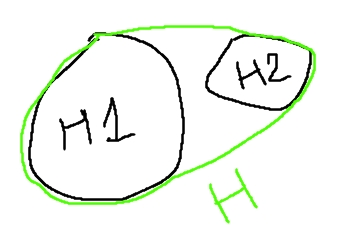
\includegraphics[width = 9cm]{Hull_merging.jpg}
    \caption{}
    \label{fig:float}
\end{figure}

Хорошо параллелится, также за $O(n) + O(nlogn)$, но с "плохими" коэффициентами.